The world around us has structure, and to an adult appears to be made
up of more-or-less well-defined objects.  How do we develop the
sophisticated perceptual judgements needed to maintain this view?
Infant research has revealed a long developmental process, during
which infant judgements converge incrementally on those of adults.
This may offer guidance to roboticists on how to construct a
sophisticated perceptual system~-- what the right modules are, how
they can be ``trained'', and how they interact.  We review aspects 
of that developmental process here.



\begin{figure}

\centerline{\includegraphics[width=0.75\columnwidth]{fig-seg}}

\caption{
%
Image segmentation and object segregation are different.  On the left,
there is a simple scenario, taken from \citeasnoun{needham01object}
(not quite the right image),
showing a rectangle attached to a yellow tube.  Two 
plausible ways to segregate this scene are shown in the middle,
depending on whether the tube and rectangle make up a single 
object.
For
comparison, automatically acquired boundaries are shown on the right,
produced using the algorithm in
\citeasnoun{felzenszwalb04efficient}. 
In image segmentation, the goal is to
produce regions that correspond to whole objects (such as the yellow
tube) or at least to object parts (such all the blue rectangle and all
the small white patches on its surface, and various parts of the
background).  Ideally, regions that extend across object boundaries
are avoided.  Then, higher-level processes need only consider merging
regions (of which there are a relatively small number) rather than
splitting regions (which requires a return to pixel-level
considerations).  
%
%
}

\label{fig:image-segmentation}

\end{figure}


In psychology, the human ability to divide a scene into a set of
discrete objects is termed ``object segregation.''  
In computer vision and robotics, there are algorithms with 
similar goals.  In practice, automatic object segregation
in unconstrained environments is not currently possible.
%
Progress has been made on a related, less ambitious problem
called ``image segmentation''.  The goal of image segmentation
is to divide an image of a scene into a set of discrete
regions, where each region corresponds to an object or 
an object part.  The distinction between this and 
segmentation is made clear in Figure~\ref{fig:image-segmentation}.
%
Image segmentation will typically produce more regions than there are
objects.  The idea is that those ``summary'' regions could then be
merged by more informed, higher level processing (although successful
algorithms for such higher level processing do not actually currently
exist for unconstrained environments).  Regions designed to be
used this way are also called ``superpixels''.
%
They can be produced by bottom-up processes that look for 
similarily in color and texture.  We give an example algorithm later
in this section.
%

For humans, visual experience is continuous, and comes from our two
eyes.  Image segmentation can be generalized to video sequences, and
to input from multiple view-points.  Real-time, robotic
implementations of image segmentation are primitive compared to
state-of-the-art off-line segmentation algorithms, and focus on simple
cases, such as colorful or moving objects.
%
However, robotic work is potentially well suited to addressing the
parts of object segregation that have been omitted from image
segmentation: specifically, the role of {\em experience} over
various time-scales.  Object boundaries are revealed in some
circumstances and obscured in others; how do we propogate this
information?  We can ask this over short time-scales, within
a working session, or over longer time-scales and ranges
of experiences.

We look at the role of experience in infants' object 
segregation skills, and work to factor experience into 
image segmentation for machine vision.


\subsection{Development of infants' object segregation skills}

It is clear that human infants learn generic principles for making
educated guesses about which surfaces belong together as part of the
same unit and which do not.  By 4 to 5 months of age, infants can
parse simple displays into units based on something like static
gestalt principles, probably some subset of these (e.g. \citeasnoun{needham98infants,needham00improvements}).

Similar results have been obtained by researchers using partly
occluded objects (Johnson--+ display??)

Initial studies indicated that infants used some collection of
features to parse the displays \cite{needham98infants,needham97object,needham98effects}; subsequent studies suggested that object shape is the key
feature that young infants use to identify boundaries between adjacent
objects \cite{needham99role}.

These principles may lead to many incorrect parsings, but they will
also provide reasonable best guess interpretations of uniform objects
in complex displays.  


Supporting a differentiation view of the development of
generalization, Bahrick's findings suggest that young (i.e.,
2-month-old) infants are more likely to generalize farther from the
specific experiences they received than infants just a few months
older (get citation).  This finding suggests that experience might
serve to initially narrow and then extend the range of stimuli over
which young children will generalize.


Infants do not come prepared to segregate objects into units that
adults would consider meaningful.  Rather, infants learn how object
features can be used to predict object boundaries.  More than twenty
years ago, \citeasnoun{kellman83perception} suggested that infants may be born
with knowledge about solid, three-dimensional objects and that this
knowledge could help them interpret portions of a moving object as
connected to other portions that were moving in unison.  However, this
assertion was put to the test by Slater and his colleagues (is this
\citeasnoun{slater90newborn}?), a test that resulted in a new conception of
the neonate's visual world.  Rather than interpreting common motion as
a cue to object unity, they interpreted the visible portions of a
partly occluded object as clearly separate from each other, even when
undergoing common motion.  This finding was important because it
revealed one way in which learning likely changes how infants
interpret their visual world.


Although adjacent objects present a very similar kind of perceptual
problem (are these surfaces connected or not), the critical components
of success might be quite different.  Early work with adjacent objects
indicated that at 3 months of age, infants tend to group all touching
surfaces into a single unit \cite{kestenbaum87perception}.
Subsequent experiments have revealed that soon after this point in
development, infants begin to analyze the perceptual differences
between adjacent surfaces and segregate surfaces with different
features (but not those with similar features) into separate units
(Needham 2000).  Although infants can use the boundary seam between
two objects as a source of information about the likely separation
between them (Kaufman \& Needham, submitted), other work comparing
boundary-occluded and fully visible versions of the same displays
suggests that boundary information is not the only information infants
use to parse the objects in a display (Needham, 1998).  

Infants also use information about specific objects or
classes of objects to guide their judgement.  
NEEDHAM, CANTLON, \& ORMSBEE 2005 (age: 8.5 months).


It might be that extensive amounts of experience are required to
`train up' this system.  However, it might also be that infants learn
on the basis of relatively few exposures to key events (Baillargeon,
1999).  This possibility was investigated within the context of object
segregation by asking how infants' parsing of a display would be
altered by a brief prior exposure to one of the objects in the test
display.



\subsection{Specific instances of experience affecting infants' segregation judgements}

In this paradigm, a test display was used that was ambiguous to
4.5-month-old infants who had no prior experience with the display.
Prior experience was given that would help disambiguate the display
for infants.  This experience consisted of a brief prior exposure
(visual only) to a portion of the test display.  If infants used this
prior experience to help them parse the test display, they should see
the display as two separate objects and look relaibly longer when they
moved as a whole than when they move separately.  Alternately, if the
prior experience was ineffective in altering infants'
interpretation of the display, they should look about equally at the
display, just as the infants in the initial study with no particular
prior experience did \cite{needham98effects}.  Prior experiences
with either portion of the test display were effective in facilitating
infants' parsing of the test display.  

However, when we introduced changes between the box seen during
familiarization and that seen as part of the test display, an
unexpected pattern emerged.  Nearly any change in the object's
features introduced between familiarization and test prevented infants
from benefitting from this prior experience.  So, even when infants
saw a blue box with yellow squares prior to testing, and the box used
in testing had white squares but was otherwise identical, they did not
apply this prior experience to the parsing of the test display.
However, infants did benefit from the prior exposure when it was not
in the features of the object but rather in its orientation 
 \cite{needham01object}.  
A change in the orientation of the box from horizontally to
vertically oriented led to the facilitation in parsing seen in some
prior experiments.  Thus, infants even as young as 4.5- to 5-months of
age know that to probe whether they have seen an object before, they
must attend to the object's features rather than its spatial
orientation \cite{needham01object}.

These results also support two additional conclusions.  First,
infants' object representations include detailed information
about the object's features.  Because infants'
application of their prior experience to the parsing of the test
display was so dependent on something close to an exact match between
the features, one much conclude that a highly detailed representation
is formed on the initial exposure and maintained during the
inter-trial-interval.  Because these features are remembered and used
in the absence of the initial item and in the presence of a different
item, this is strong evidence for infants' representational
abilities.  Secondly, 4.5-month-old infants are conservative
generalizers -- they do not extend information from one object to
another very readily.  But would they extend information from a {\bf group}
of objects to a new object that is a member of that group?


\subsection{Generalization of knowledge gained from experience}

This question was investigated by \citeasnoun{needham05infants}
in a study using the same test display and a similar procedure as in
\citeasnoun{needham01object}.  Infants were given prior experiences with collections
of objects, no one of which was an effective cue to the composition of
the test display when seen prior to testing.  A set of three similar
objects seen simultaneously prior to test did facilitate 4.5-month-old
infants segregation of the test display.  But no subset of these three
objects seen prior to testing facilitated infants' segregation of the
test display.  Also, not just any three objects functioned in this way
-- sets that had no variation within them or that were too different
from the relevant test item provided no facilitation.  Thus,
experience with multiple objects that are varied but that are similar
to the target item is important to infants' transfer of their
experience to the target display.



This finding was brought into the ``real'' world by investigating
infants' parsing of a test display consisting of a novel key
ring (Needham et al., submitted; see Figure X).  According to a strict
application of organizational principles using object features, the
display should be seen as composed of (at least) two separate
objects -- the keys on one side of the screen and the separate
ring on the other side.  However, to the extent that infants recognize
the display as a member of a familiar category -- key
rings -- they should group the keys and ring into a single unit
that should move as a whole.  Our findings indicate that by 8.5 months
of age, infants parse the display into a single unit, expecting the
keys and ring to move together.  Younger infants do not see the
display as a single unit, and instead parse the keys and ring into
separate units.  Infants of both ages parsed an altered display, in
which the identifiable portions of the key ring were hidden by
patterned covers, as composed of two separate units.  Together, these
findings provide evidence that the studies of controlled prior
exposure described in the previous section are consistent with the
process as it occurs under natural circumstances.  Infants'
ordinary experiences present them with multiple similar exemplars of
key rings, and these exposures build a representation that can then be
applied to novel (and yet similar) instances of the key ring category,
altering the interpretation that would come from featurally-based
principles alone.




\subsection{Role of behavior in the development of object segregations skills}

Evidence from of one set of studies reveals that young
infants' difficulty in collecting the relevant information
from visual displays may limit their success in these tasks (Johnson \&
Aslin 1995, \cite{johnson96perception}, then Johnson's eye tracking stuff
\cite{johnson04where} showing
that infants who look to the other side of the occluder, sampling
information from both sides of it, are the ones who perceive the
object parts as connected.  So, eye movements are an important factor
in this picture)

The changes in perception described throughout this section
do not occur in a vaccuum but rather in a
child who is also experiencing a range of other develomental changes.
One of these changes occurs in object
exploration -- infants' visual, oral, and manual
investigation of objects are showing huge improvements during this
same time period \cite{rochat89object}.  Relations between infants'
tendency to explore objects more or less actively and their accurate
parsing of an object display has been shown \cite{needham00improvements}, paving
the way for future studies of connections between object exploration
and object perception.





\begin{figure}[t]

\centerline{
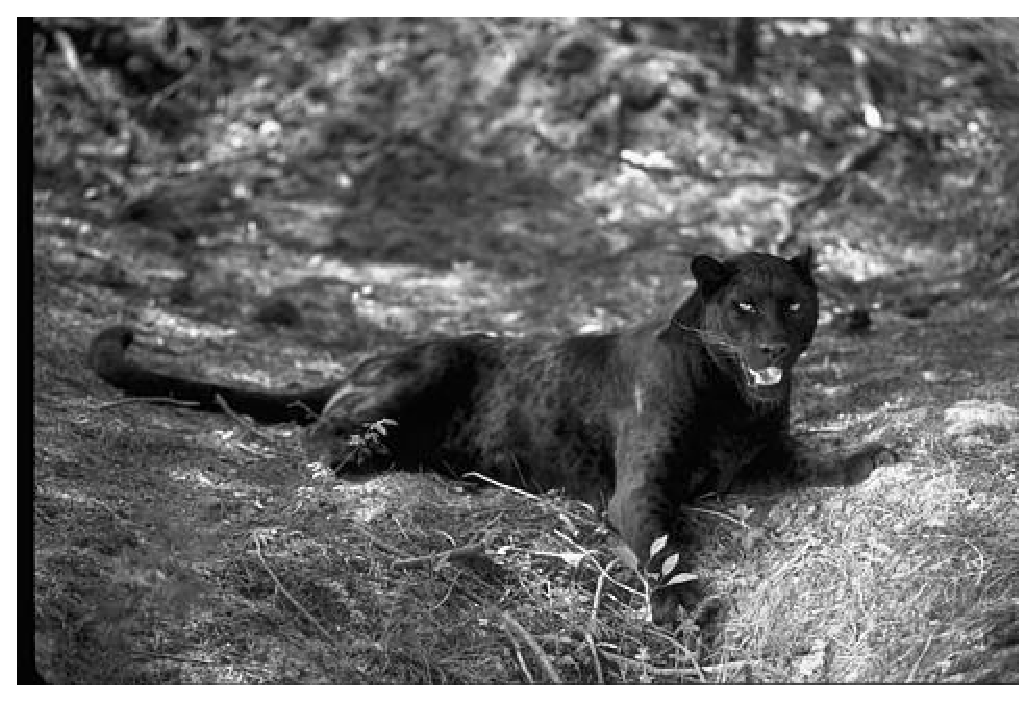
\includegraphics[width=0.3\columnwidth]{cat}
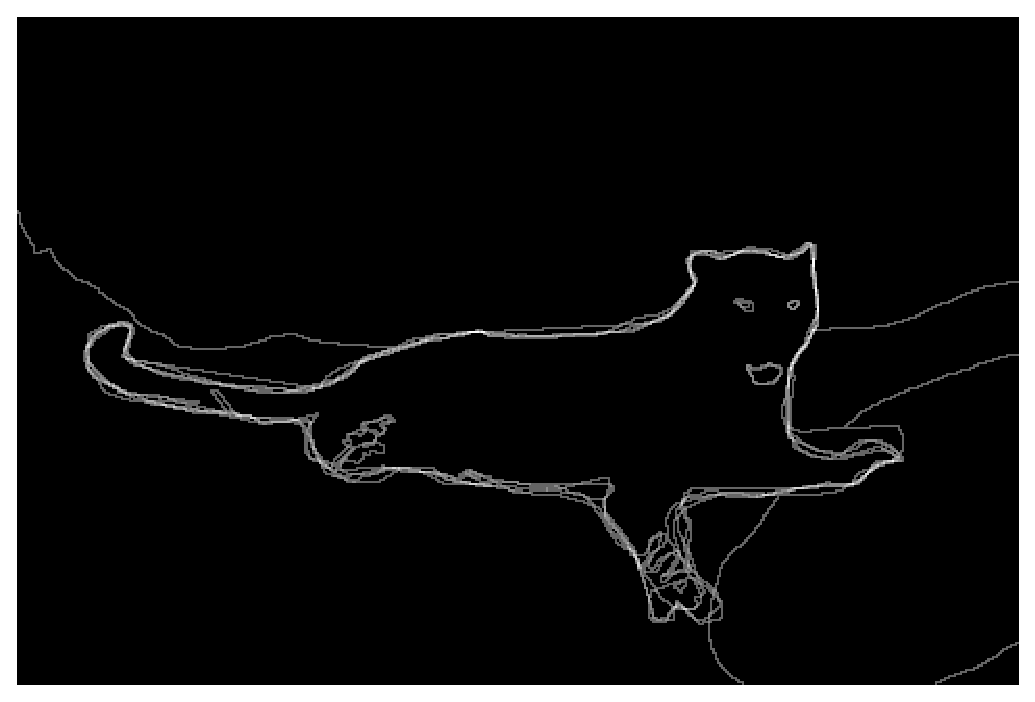
\includegraphics[width=0.3\columnwidth]{cat-human}
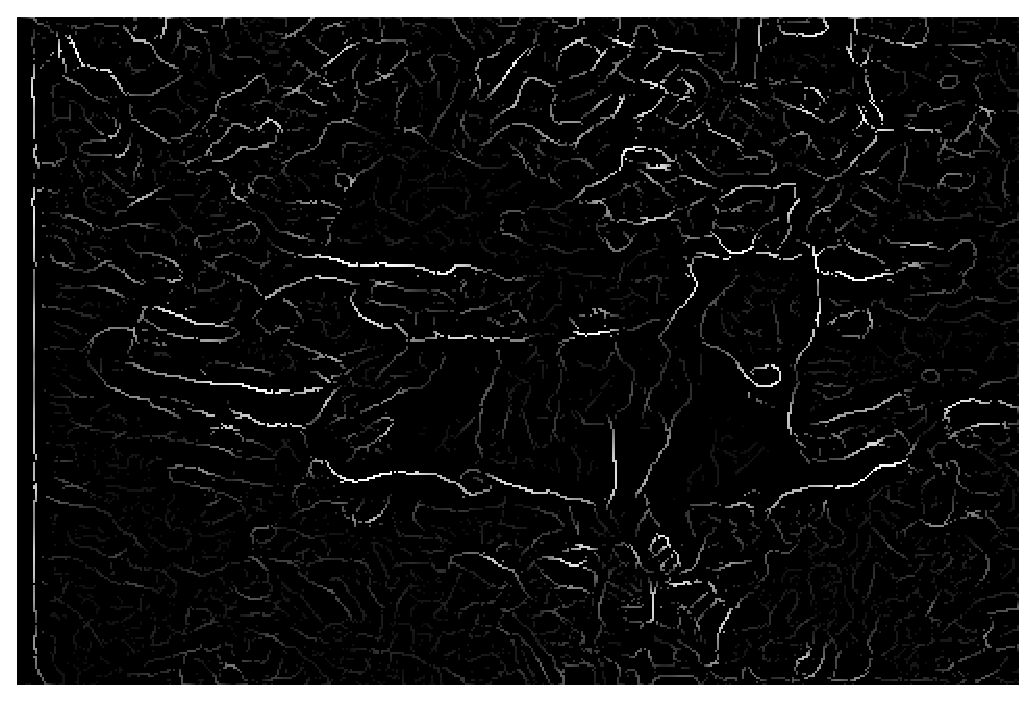
\includegraphics[width=0.3\columnwidth]{cat-machine}
}

\caption{
From [Martin et al].  Bottom-up segmentation is hard.
Image (left).  Human-labelled boundaries (middle).
Best machine segmentation of a set of algorithms (right).
}

\label{fig:segmentation-is-hard}

\end{figure}



\subsection{Object segregration in computer vision}

Object segregation is a problem of deep interest to researchers in
computer vision and robotics.  Many algorithms exist for many variants
of the problem.  
Of course, none of them even comes close to human (or
infant) performance.  
Spelke wrote in 1990:

\begin{quote}

... the ability to organize unexpected, cluttered, and
changing arrays into objects is mysterious: so mysterious
that no existing mechanical vision system can accomplish this task
in any general manner.
\cite{spelke90principles}

\end{quote}

\noindent
This is still true today.
For example, Figure~\ref{fig:segmentation-is-hard} shows the
output of a start-of-the-art algorithm for finding boundaries in images
\cite{martin04learning} compared with human performance.  This is
admittedly a particularly difficult case, but it is clear that 
a remains to
be done.


The segregation problem has been formalized in various ways.  Here is
a typical formalism (which is in fact used for many problems, not just
segregation).  There is an input image, $X$, which is a view of the
world from a camera, represented as a matrix of {\em pixels}.  Each
pixel is a simple real number representing gray-level, or a vector
representing color in RGB.
%
There is an output matrix, $Y$, where each pixel is replaced by
a {\em label}, a simple integer.  Pixels corresponding to the 
same label are considered to belong to the same region.

We can construct an {\em energy function} that evaluates the quality
of the labelling in terms of the input.  This function is designed so
that by minimizing it (by changing our choice of labelling, $Y$), we
get good results.  The energy function can be broken into two
parts:

\begin{displaymath}
%
E(X,Y) = E_{smooth}(Y) + E_{data}(X,Y)
%
\end{displaymath}

$E_{smooth}$ measures how well our labelling matches the
expectation that neighboring pixels should generally have the
same label (belong to the same region).
As far as this term is concerned, the smoother the better -- there is
a cost for neighboring pixels being assigned different labels.
$E_{data}$ measures conflicts between the labelling and the data (for
example, assigning equal labels to pixels with very different
appearance.

Particular forms of the energy function admit of efficient 
approximate solutions, and have been the topic of much research.
%
The energy function is usually {\em local} -- terms are computed 
based on comparisons between small neighborhoods of pixels.
%
This formalization works well with grouping based on local
cues -- similarity in brightness, color, and some forms of texture.
It is less suited to ``shape'' cues.


Object boundaries are much more difficult to detect reliably than might be 
expected from introspection.
Statistics learned from data has been shown to be useful
\cite{konishi03statistical}.  Large databases of 
human-labelled boundaries are being collected and
used to train better systems
\cite{martin04learning}.
%
Such databases are extremely time-consuming to produce.
%
\citeasnoun{ross05learning} developed a system that performs
segmentation based on static cues (color, texture, brightness)
using statistics learned from motion segmentation.
In principle, motion is a very powerful cue for
segmentation; certainly that is the case for infants
[CITE].
%
Progress is being made on motion segmentation, both 
in improving its accuracy and increasing its efficiency
 \cite{cremers05motion,fowlkes04spectral,smith03motion,smith04layered}.
%
Currently, accurate motion segmentation is 
computationally challenging in unconstrained environments.


\subsection{Object segregration in robotics}

For object segregation in robotics, the biggest challenge is real-time
operation~-- many state-of-the-art segmentation algorithms are
unacceptably slow.  On the other hand, robots have two very
advantageous properties.  
%
The first is
{\em locality}~-- a robot exists at a certain time and place, and the
set of objects it must work with at any moment is bounded.  
%
The second is
{\em continuity}~-- a robot has a longer term relationship with
the objects embedded in its sensors than, for example, a car 
detector searching through images on the web.
%
These conditions encourage approaches to object segregation
that are experience-driven.
%
The key to such approaches is to find
opportunities in the robot's experience where the
true boundary of an object can be reliably inferred,
and then determine correlates of the boundary that 
are available more generally.
%
For example, \citeasnoun{fitzpatrick03grounding} used
a very specific condition (objects being hit by
people or the robot itself) to extract good
motion-based object boundaries; surface features
of the object could then be used to segregate that
object out in static presentations \cite{fitzpatrick03object}.
\citeasnoun{arsenio05exploiting} used rhythmic motion
of objects to segment their boundaries both in
visually and acoustically.
%
Arsenio (CITE THESIS) developed a set of techniques for acquiring all
sorts of segmentations.  Some methods work for small, grasp-size
objects, others work for large background objects like walls or
tables.





\begin{figure}[t]

\centerline{

\includegraphics[width=0.75\columnwidth]{fig-robot}
}

\caption{
%
Object segregation based on specific object experience.  The robot
detects object boundaries experimentally \cite{fitzpatrick03object}.
It searches for good features of the object that contrast with other
objects, and that are stable with respect to certain geometric
transformations.  These features are then used to jointly detect
and segment the object in future views.  Left: the robot.
Middle: segmentations of an object derived opportunistically
from experience.  Right: the robot's perspective on a scene 
containing the object on a table.  The object is correctly segmented;
the table is completely ignored.
%
}

\label{fig:robot}

\end{figure}



These systems are limited in how information from experience can be
generalized.  In \citeasnoun{fitzpatrick03object}, for example,
information is either pooled across all contexts (in the case of edge
appearance modeling) or intended to be specific to one particular
object.  There is no notion of object category.
%
In this respect, Needham's results on generalizations are
very interesting, in possibly pointing a way forward.


\subsection{Discussion of available cues and their reliability}

Using color and texture features is perhaps limiting, since they
are relatively accidental.  Infants seem to ignore them for
certain purposes [CITE].
%
Physical boundaries are functions of object shape.  But object shape
is difficult to recover in natural scenes.
%
One correlate of shape is object contour.  In a comparision between
contour-based and appearance-based methods for object categorization
\cite{leibe03analyzing}, shape-based cues are shown to be
particularly useful for categorization.
Ditto \cite{lecun04learning}.
For specific tasks, color/texture can be useful, but for 
generic tasks they are a distraction.

Biologically inspired mechanisms are competitive:
Serre's model for recognition \cite{serre05object}.


Discuss value of cues in terms of information content (how many bits),
accessibility (how hard is it to actually estimate those bits
correctly), constancy over different timescales and variations.

Luminance, color, texture, motion, shape, location, seams, stereo,
shadow.

For segregation and (a little bit) for recognition.

Pending:

\cite{swain91color}.

\cite{schiele00recognition}.

\cite{lowe04distinctive}

\cite{felzenszwalb04efficient}

maturation v experience \cite{quinn05learning}.

In figure, using \cite{felzenszwalb04efficient}.

\cite{gibson88exploratory}

\cite{spelke90principles}

\cite{martin01database}

The Torralba-led contextual approach.


shadows and interreflections for object contact
\cite{madison01use}.


Stereo review -- depth maps, making progress
\cite{scharstein02taxonomy}

theoretically, more info at corners \cite{feldman05information}

connectionist model
\cite{mareschal02learning} --

\begin{quote}

For infants younger than 6 months, common motion of surfaces that lead
behind an occluder is both necessary and sufficient to specify their
unity. Only after 6 months do infants utilize additional sources of
information for unity, such as surface appearance, and edge and
surface orientation. \cite{mareschal02learning}

\end{quote}


Wilcox on the why \cite{wilcox99object}.  Maybe don't get
``sufficient contrastive evidence within the context of
occlusion events''.


Also of interest:

\begin{quote}

In contrast, infants first demonstrate color constancy around 4-5
months of age, and then only under limited conditions ( Dannemiller
and Dannemiller).

Finally, because form features are amodal - they can be
experienced visually, orally, or haptically - they may be more
salient to young infants.

\end{quote}

Color constancy in 4-month olds: \cite{dannemiller87test} -- some 
limitations.

Nifty: not age at which feature is detectable, but the actual
info it carries, that affects at what age it gets used for
individuation -- luminance test \cite{woods05infants}.

Infants' formation and use of categories to segregate objects 
\cite{needham05infants}.

Feature priming -- \cite{wilcox04priming}


stacked objects sharing a boundary are harder
to segregate than the same two objects
side by side?  attrib to needham by xu,
paintbrush/keyring.


texture hint \cite{johnson96perception}?

depth placement and contour ownership?

\begin{quote}

Spelke noted that any mechanism for segmenting the visual array
into objects must ascertain the boundaries of adjacent objects,
the complete shapes of partly occluded objects, and the continued
existence of objects that are no longer visible.
(Johnson 1996 quoting Spelke 1990 - get original)

\end{quote}

Relatable edges: can be connected with a smooth monotic
curve behind occluder.

Including and excluding ``perceptual completion.''

Interesting developmental progressions, e.g. of perception
of transparency: \cite{johnson00infants}


Some quick learning shown via eye movements \cite{johnson03development}.


There is a difference of concerns.  In infant research, have
at least two instances of scenarios where infant has
plastic perception.

In fact habituation paradigm requires a form of short-term
plasticity. 


\cite{prechtl01role} influence of vision on early motor 
development.

\subsection{Active vision}

\cite{bajcsy88active,aloimonos87active,ballard91animate}

driven by uncertainty \cite{whaite97autonomous}, 
extensions in SLAM.

Computational color constancy isn't that great
\cite{barnard02comparison}.

Habituation -- how does it really work \cite{sirois02models}.
Attraction to familiar; attraction to novelty.
How to build such a system?

sensorimotor account \cite{oregan01sensorimotor};
infant representation a challenge.  Controversy.

Image parsing \cite{tu05image}.

